\section{Desenvolvimento Teórico}
\subsection{Velocidade da Luz}
O feixe de luz que sai do laser é refletido em um ângulo $\theta$ com a reta normal do espelho rotatório ($MR$), como mostrado na $Figura 1$, em direção ao ponto $S$ do espelho fixo ($MF$). Ao passo que o espelho $MR$ rotaciona, sua reta normal irá variar em ângulo  $\Delta \theta$, resultando em um novo ângulo de incidência $\theta1$. O feixe incidirá então no ponto $S1$ do espelho $MF$.
\begin{figure}[!ht]
	\centering
	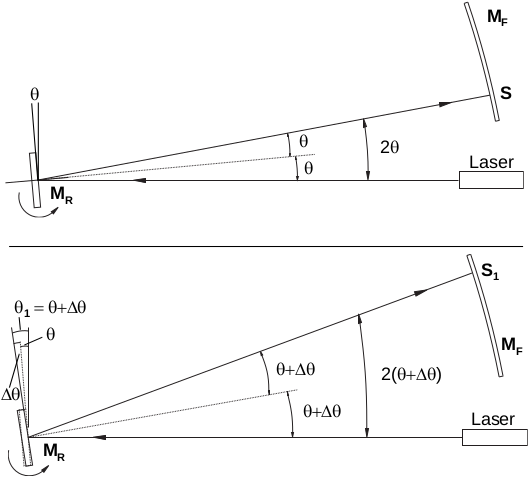
\includegraphics[scale=0.4]{2.png}
	\caption{Diagrama do caminho óptico percorrido pelo feixe e detalhe da diferença angular decorrente da rotação do espelho $MR$}
\end{figure} 
Sendo $D$ a distância entre os espelhos, a diferença de caminho entre os feixes é dada por:

\begin{equation}
	S1-S = D(2\theta1 - 2\theta)=D[2(\theta+\Delta\theta)-2\theta]= 2D\Delta		\theta
\end{equation}
Uma análise semelhante pode ser empregada na seguinte montagem:

\begin{figure}[!ht]
	\centering
	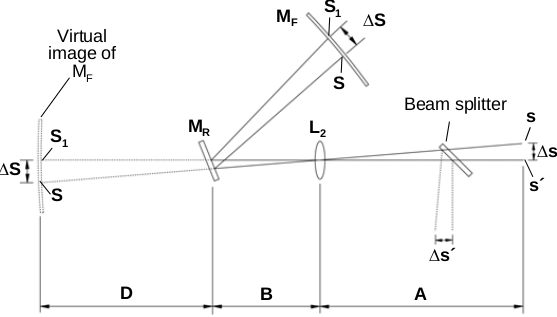
\includegraphics[scale=0.4]{3.png}
	\caption{Diagrama do caminho óptico semelhante ao arranjo experimental \cite{PASCO}}
\end{figure}
Onde o deslocamento do ponto imagem ($\Delta S'$) decorrente da rotação do espelho $MR$ é igual ao deslocamento $\Delta S$ da imagem virtual no espelho $MF$, a qual é determinada pela relação:

\begin{equation}
	\Delta S'= \Delta S=(-i/o)\Delta S
\end{equation}
Em que $i$ é a distância da imagem até a lente e $o$ a distância do objeto até a mesma ($L2$). Pela $Figura2$ obtem-se que:

\begin{equation}
	(-i/o)\Delta S=\frac{A}{D+B}\Delta S
\end{equation}
 
Substituindo o valor de $\Delta S$ obtido na eq. $1$:

\begin{equation}
	\Delta S'=\frac{2DA\Delta\theta}{D+B}
\end{equation}

Sabendo-se que o ângulo $\Delta\theta$ depende da velocidade de rotação ($\omega$) do espelho $MR$, do trajeto do feixe entre os espelhos ($2D$) e da velocidade $c$ da luz, resulta:

\begin{equation}
	\Delta\theta=\frac{2D\omega}{c}
\end{equation}

Com a igualdade da eq. $4$

\begin{equation}
	\Delta S'=\frac{4D^{2}A\omega}{c(D+B)}
\end{equation}

Isolando-se $c$:

\begin{equation}
	c=\frac{4D^{2}A\omega}{(D+B)\Delta S'}
\end{equation}
substituindo $\omega$ por $2\pi f$
\begin{equation}
	c=\frac{8D^{2}A\pi f}{(D+B)\Delta S'}
\label{eq:C}
\end{equation}
Variando então os parâmetros $\omega$ e, consequentemente, $\Delta S'$ e conhecendo os demais valores das constantes, é posível calcular a velocidade $c$ da luz.

\subsection{Desvios}
\subsubsection{Desvio de Medidas Diretas}
Para este experimento, tem-se como medidas diretas, as distancias entre os espelhos e lentes, e a variação da posição do feixe de luz no microscópio. Para as medidas de distancia foi utilizada uma trena com o erro associado de $0,005m$ e para o $\Delta s$ tem-se o erro de $2,5mm$,pois a menor variação que é possivel medir é de $5mm$.
\subsubsection{Desvio de Medidas Indiretas}
Para o calculo de Velocidade da luz é utilizada a equação \ref{eq:C} e para o cálculo dos erros, é aplicado o logaritimo neperiano em ambos os lados da equação, tornando-se:

\begin{equation}
	ln(c)=ln(\frac{8D^{2}A\pi f}{(D+B)\Delta S'})
\end{equation}

e utilizando a propriedade de divisão de logaritimos, é obtido

\begin{equation}
	ln(c)=ln(8D^{2}A\pi f)-ln((D+B)\Delta S')
\end{equation}
\begin{equation}
	ln(c)=ln(8A) + 2ln(D) - [ln(D+B)+ln(\Delta S)]
\end{equation}
diferenciando a equação
\begin{equation}
	\frac{dc}{c}=\frac{dA}{8A} + \frac{2dD}{d} + \frac{dA}{A+B} + \frac{dB}{A+B}+\frac{d\Delta S}{\Delta S}
\end{equation}
e fazendo $d\rightarrow \delta$ para poder ser aplicado os erros medidos experimentalmente. Onde $\delta$ representa o erro associado.
\begin{equation}
	\frac{\delta c}{c}=\frac{\delta A}{8A} + \frac{2\delta D}{d} + \frac{\delta A}{A+B} + \frac{\delta B}{A+B}+\frac{\delta \Delta S}{\Delta S}
\label{eq:err}
\end{equation}
